\chapter{Anhang}

\section{Verwendete Hilfsmittel}
In der Tabelle \ref{tab:tooling} sind die im Rahmen der Bearbeitung des Themas der \IthesisKindDE~verwendeten Werkzeuge und Hilfsmittel aufgelistet.

\begin{table}[h!]
\caption{Verwendete Hilfsmittel und Werkzeuge}
\begin{tabular}{|l|l|}
\hline 
\rowcolor{lightgray} Tool & Verwendung \\
\hline
\LaTeX & Textsatz- und Layout-Werkzeug verwendet zur Erstellung dieses Dokuments \\
\hline
 & \\
\hline
\end{tabular}
\label{tab:tooling}
\end{table}

\section{Abbildungen}

\begin{figure}[htbp]
    \begin{center}
        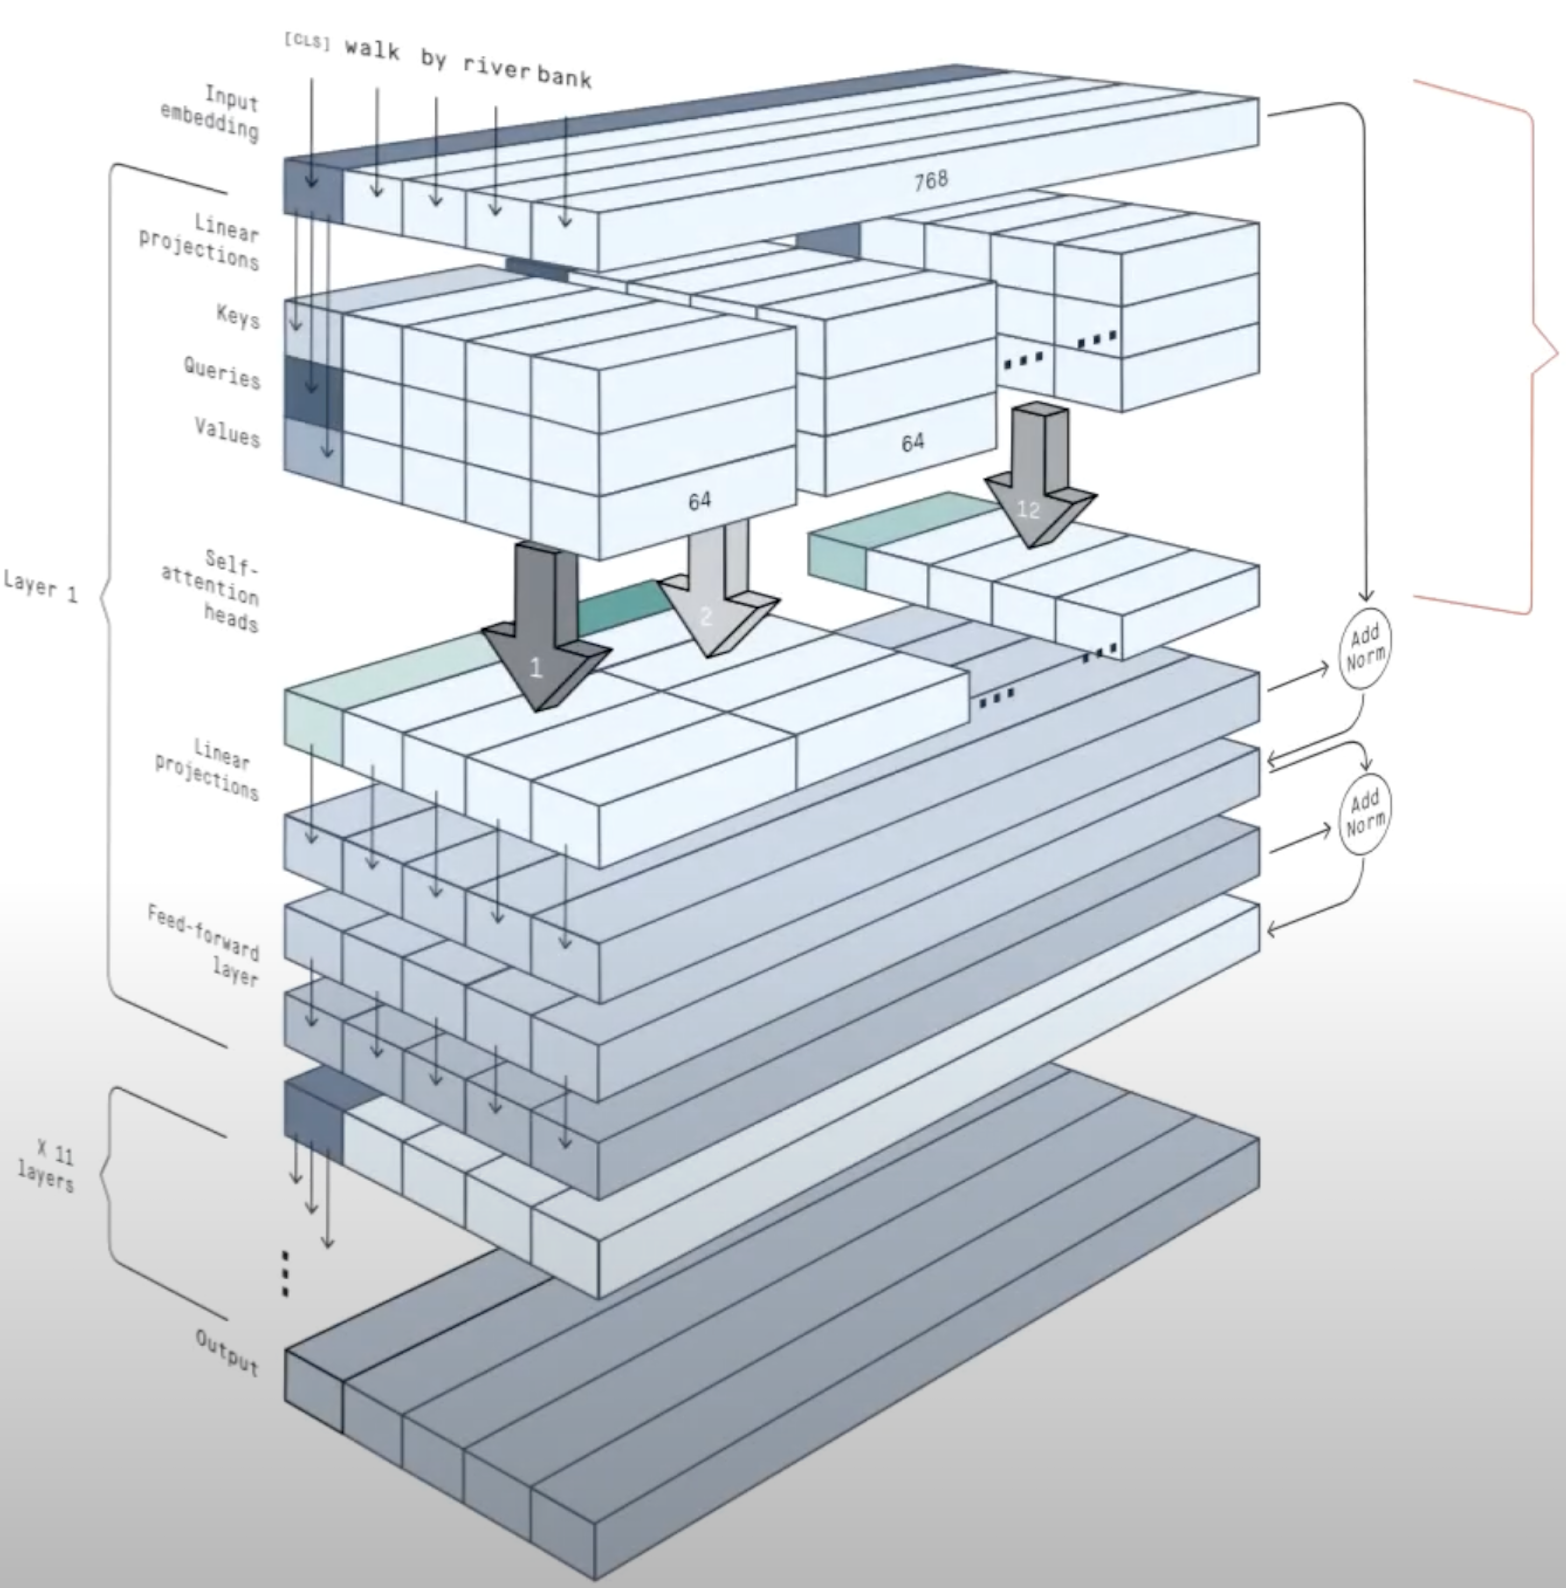
\includegraphics[scale=0.5]{static/BERT_visualization.png}
        \caption{\label{fig:BERT_visualization} Architektur des BERT Modells \cite{peltarion2020bert}}
    \end{center}
\end{figure}

\begin{figure}[htbp]
    \begin{center}
        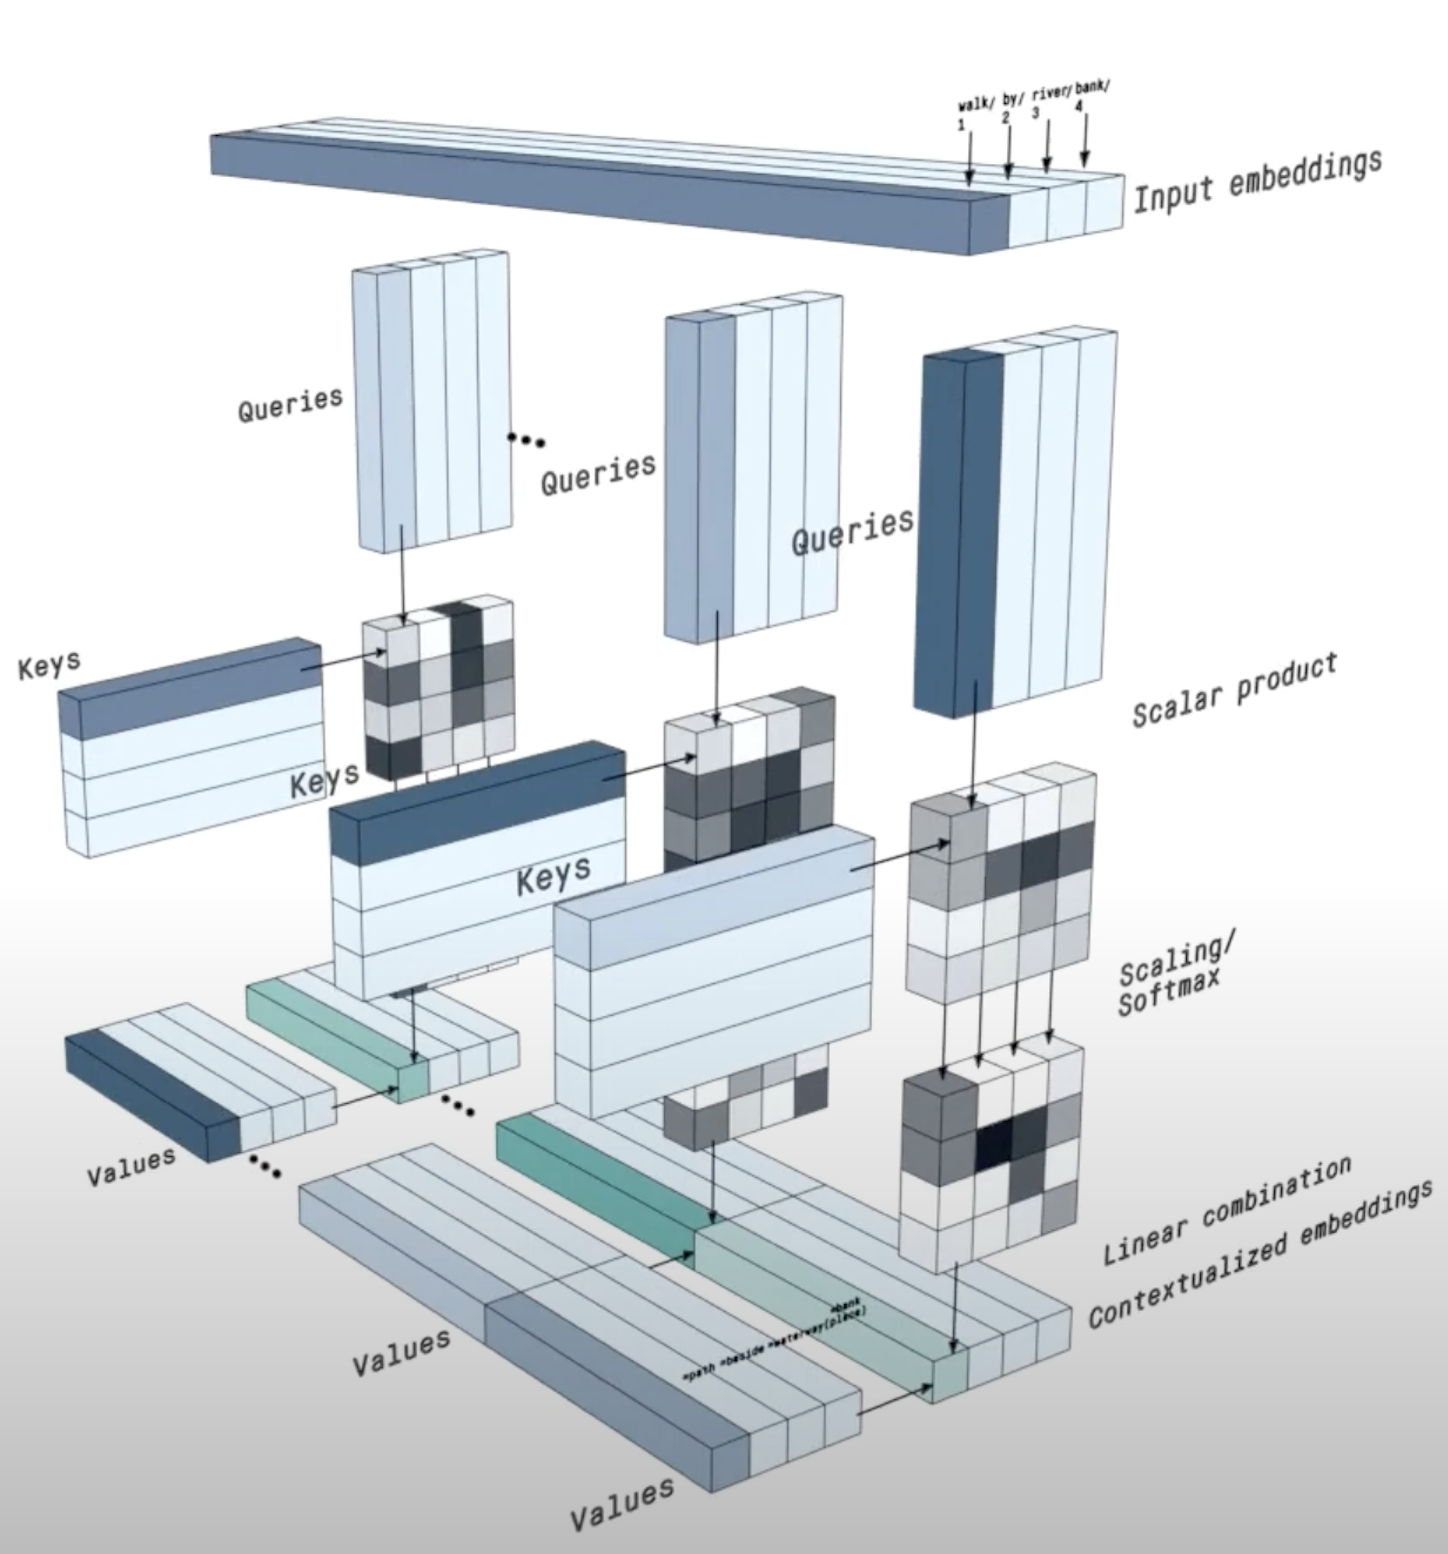
\includegraphics[scale=0.5]{static/multi-head_attention_visualization.png}
        \caption{\label{fig:multi_head_attention_visualization} Multi-Head Attention \cite{peltarion2020bert}}
    \end{center}
\end{figure}

\begin{sidewaystable}[htbp]
\centering
    \begin{tabular}{|p{3.5cm}|p{2.8cm}|p{2.8cm}|p{2.8cm}|p{2.8cm}|p{2.8cm}|}
        \hline
        \textbf{Merkmal} & \textbf{BERT Base} & \textbf{RoBERTa\newline Base} & \textbf{RoBERTa Large} & \textbf{XLM-RoBERTa Base} & \textbf{XLM-RoBERTa Large} \\
        \hline
        \textbf{Hidden Size} & 768 & 768 & 1024 & 768 & 1024 \\
        \hline
        \textbf{Anzahl Layer} & 12 & 12 & 24 & 12 & 24 \\
        \hline
        \textbf{Anzahl Attention Heads} & 12 & 12 & 16 & 12 & 16 \\
        \hline
        \textbf{Vocab Size} & 30,522 & 50,265 & 50,265 & 250,002 & 250,002 \\
        \hline
        \textbf{Spezialisiert auf} & Masked LM & Masked LM & Masked LM & Multilinguales Masked LM & Multilinguales Masked LM \\
        \hline
        \textbf{Sprachumfang} & Englisch & Englisch & Englisch & Multilingual & Multilingual \\
        \hline
    \end{tabular}
\caption{Vergleich der verschiedenen BERT- und RoBERTa-Modelle}
\label{tab:bert_models}
\end{sidewaystable}

\begin{figure}[htbp]
    \begin{center}
        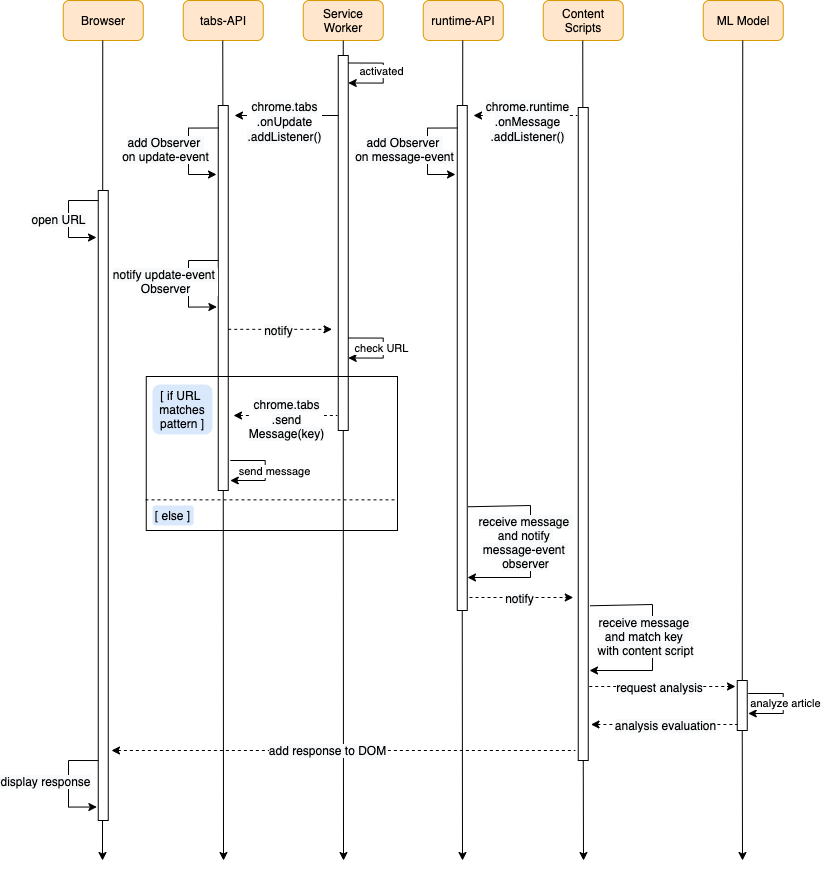
\includegraphics[scale=0.5]{diagrams/hauptkomponente_sequenzdiagramm.png}
        \caption{\label{fig:seq_hauptkomponente} Sequenzdiagramm Webagent}
    \end{center}
\end{figure}

